% Folien 6–13: Bildfrage, mathematische Idee und eigener Versuch.
\begingroup
% Auf die Konzeptfolien begrenzt; die abgenommenen Folien behalten ihre Typografie.
\renewcommand{\small}{\fontsize{9.2}{11}\selectfont
  \setlength{\abovedisplayskip}{4pt}\setlength{\belowdisplayskip}{4pt}
  \setlength{\abovedisplayshortskip}{2pt}\setlength{\belowdisplayshortskip}{3pt}}
\setlength{\parskip}{1.5pt}
\newcommand{\tafelverweis}[2]{\hyperlink{tafel#1}{\textcolor{sea}{\scriptsize Tafelbild #1 · #2}}}
\newcommand{\editorauftrag}[3]{%
  \vfill\par\smallskip
  {\small\href{\workshopurl editor.html?demo=#2}{\textcolor{sea}{\textbf{Im Editor: Demo #1 öffnen → START wählen.}}}\par}
  {\small\textbf{Ausprobieren:} #3\par}%
}

\begin{frame}[label=pixelprinzip]{Ein Bild – viele Pixel}
\small
\tagline{Eine Vorschrift für jedes Pixel}\par\vspace{3mm}
\begin{columns}[c,onlytextwidth]
\begin{column}{.46\textwidth}
\begin{tikzpicture}[scale=.72]
\fill[sea!25] (3,2) rectangle (4,3);
\draw[step=1,muted!50] (0,0) grid (7,4);
\draw[thick] (0,0) rectangle (7,4);
\draw[-{Stealth}] (0,-.35)--(7.4,-.35) node[right] {$x$};
\draw[-{Stealth}] (-.35,0)--(-.35,4.4) node[above] {$y$};
\node[below left,font=\small] at (0,0) {$(0,0)$};
\node[below,font=\small] at (6.4,-.35) {$W$};
\node[left,font=\small] at (-.35,3.7) {$H$};
\fill[accent] (3.5,2.5) circle (3pt);
\node[above right,font=\small] at (3.5,2.5) {$(x,y)$};
\end{tikzpicture}
\end{column}
\begin{column}{.49\textwidth}
Dieselbe Berechnung wird für jede Pixelposition ausgeführt.
\[\boxed{\text{Farbe}=f(x,y,t)}\]
{\small
\frag{fragCoord}: Position $(x,y)$ des Pixels.\par
\frag{iResolution.xy}: Bildbreite $W$ und Höhe $H$.\par
\frag{iTime}: Zeit $t$ seit dem Start.\par\medskip
Ein \textbf{Fragment-Shader} berechnet daraus Rot, Grün und Blau für dieses Pixel.}
\end{column}
\end{columns}
%\vfill
%{\small\textbf{Zum Start:} Wir geben jedem Pixel dieselbe Farbe. Was braucht die Berechnung dafür?\par}
%\tafelverweis{1}{Pixel, Position und Bildgröße}
\end{frame}

\begin{frame}[fragile,label=pixelvorlage]{Unsere Pixel-Vorlage}
\small
\tagline{Vom Programm zur Farbe}\par\vspace{2mm}
\begin{columns}[T,onlytextwidth]
\begin{column}{.56\textwidth}
\begin{block}{Diese Funktion wird für jedes Pixel ausgeführt}
\begin{verbatim}
void mainImage(out vec4 fragColor,
               in vec2 fragCoord)
{
    vec3 color = vec3(1.0);
    fragColor = vec4(color, 1.0);
}
\end{verbatim}
\end{block}
\end{column}
\begin{column}{.40\textwidth}
{\small
\textbf{Eingabe:} \frag{fragCoord} ist die aktuelle Pixelposition.\par\medskip
\textbf{Farbe:} \frag{vec3(1.0)} steht für $(1,1,1)$: Weiß.\par\medskip
\textbf{Ausgabe:} \frag{fragColor} erhält RGB und die Deckkraft. Die letzte \frag{1.0} bedeutet vollständig deckend.\par\medskip
Die Position wird hier noch nicht benutzt: Alle Pixel werden weiß.}
\end{column}
\end{columns}
%\vfill
%{\small Wir programmieren auf der \textbf{Workshopwebsite}. Die Vorlage funktioniert auch in ShaderToy.\par}
%\tafelverweis{1}{Die Schnittstelle zur Pixelberechnung}
\end{frame}

\section{Demos}
\begin{frame}[label=demo1]{Wie verändert sich eine Farbe?}
\small
\demoheader{1 · Farbe und Zeit}
\begin{columns}[T,onlytextwidth]
\begin{column}{.46\textwidth}
\begin{minipage}{.82\linewidth}\rgbfuellanzeige\end{minipage}\par
{\small $\text{Farbe}=(R,G,B)$ mit Anteilen von 0 bis 1.\par
$(0,0,0)$: Schwarz; $(1,1,1)$: Weiß.\par
%Ohne Positionsabhängigkeit gilt die Farbe überall.
}
\end{column}
\begin{column}{.50\textwidth}
{\small\textbf{Eine Schwingung als Farbanteil}\par}
\begin{tikzpicture}[x=.78cm,y=1.65cm]
\draw[-{Stealth}] (0,0)--(6.7,0) node[right] {$t$};
\draw[-{Stealth}] (0,0)--(0,1.2) node[above] {$R(t)$};
\draw[muted!40,dashed] (0,.5)--(6.3,.5);
\draw[red,thick,domain=0:6.283,samples=70] plot (\x,{.5+.5*sin(\x r)});
\node[left,font=\scriptsize] at (0,0) {0};
\node[left,font=\scriptsize] at (0,1) {1};
\end{tikzpicture}
{\small
\[\sin(t)\in[-1,1]\quad\Rightarrow\quad R(t)=\tfrac12+\tfrac12\sin(t)\in[0,1]\]
%\frag{iTime} liefert $t$ in Sekunden. Grün und Blau schwingen zeitversetzt.\par
%Weiß → Violett → Koralle → Farbwechsel.
}
\end{column}
\end{columns}
%\editorauftrag{1}{00-konstante-farbe}{Setzt alle drei Anteile auf 0. Welche Farbe entsteht? Verändert danach einen Anteil.}
%\tafelverweis{2}{RGB und Sinus}
\end{frame}

\begin{frame}[label=demo2]{Wie wird die Position zu einem Farbanteil?}
\small
\demoheader{2 · Pixelposition und Farbverlauf}
\begin{columns}[T,onlytextwidth]
\begin{column}{.46\textwidth}
\begin{tikzpicture}[scale=.78]
\draw[thick] (0,0) rectangle (6,3.5);
\draw[-{Stealth}] (0,0)--(6.4,0) node[right] {$x$};
\draw[-{Stealth}] (0,0)--(0,3.9) node[above] {$y$};
\fill[accent] (3.6,2.1) circle (3pt);
\draw[dashed,muted] (3.6,0)--(3.6,2.1)--(0,2.1);
\node[above right,font=\small] at (3.6,2.1) {$(x,y)$};
\node[below left,font=\small] at (0,0) {$(0,0)$};
\node[below,font=\small] at (6,0) {$W$};
\node[left,font=\small] at (0,3.5) {$H$};
\end{tikzpicture}\par
{\small \frag{fragCoord} liefert $(x,y)$;\par \frag{iResolution.xy} liefert $(W,H)$.}
\end{column}
\begin{column}{.50\textwidth}
{\small\textbf{1 · Auf die Bildgröße beziehen}}
\[u=\frac{x}{W},\qquad v=\frac{y}{H}\]
{\small Die Positionsfarbe $(u,v,0)$ zeigt $x$ als Rot und $y$ als Grün.\par\medskip
\textbf{2 · Mit der Position zwei Farben mischen}}
\[C=(1-u)\,C_{\text{links}}+u\,C_{\text{rechts}}\]

\includegraphics[width=\linewidth,height=.65cm]{folien/bilder/demo-ziele/01-pixelposition-und-normalisierung.png}\par
{\scriptsize $u=0$\hfill $u=\tfrac12$\hfill $u=1$}\par
{\small Diese Mischung heißt im Code \frag{mix}.}
\end{column}
\end{columns}
%\editorauftrag{2}{01-pixelposition-und-normalisierung}{Verwendet beim Mischen \frag{uv.y} statt \frag{uv.x}. In welche Richtung läuft der Verlauf?}
%\tafelverweis{3}{Normieren und Farben mischen}
\end{frame}

\begin{frame}[label=demo3]{Wie werden aus Abständen Formen?}
\small
\demoheader{3 · Kreis und bewegte Metaballs}
\begin{columns}[T,onlytextwidth]
\begin{column}{.59\textwidth}
{\small\textbf{1 · Bildmitte als Ursprung, gleiche Einheiten}}
\[\vec p=\frac{(x,y)-\tfrac12(W,H)}{H}\]
{\small Beide Achsen durch $H$ teilen: Der Kreis bleibt rund.\par\medskip
\textbf{2 · Mit Pythagoras innen und außen unterscheiden}}
\[d^2=p_x^2+p_y^2=\operatorname{dot}(\vec p,\vec p),\quad d^2<r^2\]
{\small\textbf{3 · Abfallende Felder addieren}}
\[E_i=\frac{0{,}035}{d_i^2+0{,}01},\qquad E_1+E_2>1\]
{\small $d_i$ ist der Abstand zum jeweiligen Zentrum. $0{,}01$ verhindert Division durch null. Über der Schwelle entsteht das Objekt.}
\end{column}
\begin{column}{.37\textwidth}

\includegraphics[width=.58\linewidth]{folien/bilder/demo-ziele/03-kreis-und-quadrierter-abstand-kreis.png}\par
{\scriptsize Ein Kreis durch den Radiusvergleich.}\par\medskip

\includegraphics[width=.58\linewidth]{folien/bilder/demo-ziele/03-kreis-und-quadrierter-abstand.png}\par
{\scriptsize Die Feldsumme verbindet die Formen.}\par\smallskip
%{\small ZIEL: Sinus bewegt die Zentren.}
\end{column}
\end{columns}
%\editorauftrag{3}{03-kreis-und-quadrierter-abstand}{Ändert im Stand „Kreis“ den Radius. Was passiert beim Verbreitern der Vorschau?}
%\tafelverweis{4}{Koordinaten und Kreis}\hspace{4mm}\tafelverweis{5}{Felder und Schwelle}
\end{frame}

\begin{frame}[label=demo4]{Wie hält ein Punkt sanft an?}
\small
\demoheader{4 · Polynome für Bewegung und Farbe}
\begin{columns}[T,onlytextwidth]
\begin{column}{.46\textwidth}
\begin{tikzpicture}[x=4.4cm,y=2.3cm]
\draw[-{Stealth}] (0,0)--(1.15,0) node[right] {$t$};
\draw[-{Stealth}] (0,0)--(0,1.18) node[above] {$s(t)$};
\draw[muted,dashed,thick] (0,0)--(1,1);
\draw[sea,very thick,domain=0:1,samples=60] plot (\x,{3*\x^2-2*\x^3});
\draw[accent,thick,domain=0:1,samples=60] plot (\x,{6*\x^5-15*\x^4+10*\x^3});
\node[below,font=\small] at (1,0) {1};\node[left,font=\small] at (0,1) {1};
\end{tikzpicture}\par
{\small $t\in[0,1]$: Fortschritt auf einer Kante.\par
Die \textbf{Steigung} bestimmt die Geschwindigkeit. Die Anfangs- und Endpunkte bleiben dieselben.}
\end{column}
\begin{column}{.50\textwidth}
{\small
\textcolor{muted}{\textbf{Linear:}} $s(t)=t$\par
Start und Halt sind abrupt.\par\medskip
\textcolor{sea}{\textbf{Smoothstep:}} $s(t)=3t^2-2t^3$\par
$s(0)=0$, $s(1)=1$ und $s'(0)=s'(1)=0$: Die Geschwindigkeit geht auf null.\par\medskip
\textcolor{accent}{\textbf{Smootherstep:}} $s_2(t)=6t^5-15t^4+10t^3$\par
Zusätzlich geht die Beschleunigung an den Enden auf null.}
\[P(t)=(1-s(t))A+s(t)B\]
{\small Dieselbe Kurve mischt im Halt die Farbe:\par Schwarz → Eckfarbe → Schwarz.\par\smallskip
%\textbf{Vorbereitet:} Raute, Haltephasen und Kanon.
}
\end{column}
\end{columns}
%editorauftrag{4}{05-polynom-und-weiche-kante}{Vergleicht bei zwei Punkten LERP und Smoothstep: Bewegung und Farbwechsel.}
%\tafelverweis{6}{Interpolation, Polynome und Kanon}
\end{frame}

\begin{frame}[label=demo5]{Wie wird Zufall zu einem gestaltbaren Muster?}
\small
\demoheader{5 · Mit Rauschen gestalten}
\begin{columns}[T,onlytextwidth]
\begin{column}{.30\textwidth}
{\small\bfseries 1 · Unabhängige Pixelwerte}\par
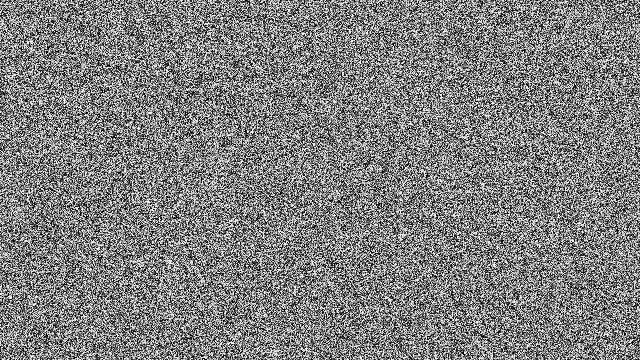
\includegraphics[width=\linewidth,trim=0bp 75bp 0bp 75bp,clip]{folien/bilder/demo-ziele/08-value-noise-zufall-pro-pixel.png}\par
{\scriptsize Gleicher Ort → gleicher Wert.}
\end{column}
\begin{column}{.30\textwidth}
{\small\bfseries 2 · Gitterwerte glatt mischen}\par

\includegraphics[width=\linewidth,trim=0bp 75bp 0bp 75bp,clip]{folien/bilder/demo-ziele/08-value-noise-value-noise.png}\par
{\scriptsize Value Noise: vier Eckwerte je Zelle.}
\end{column}
\begin{column}{.30\textwidth}
{\small\bfseries 3 · Eine andere Rauschbasis}\par
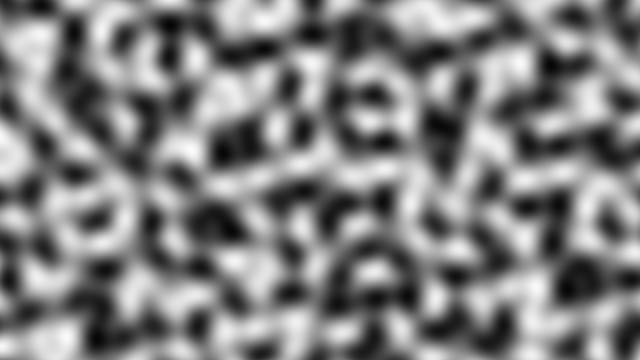
\includegraphics[width=\linewidth,trim=0bp 75bp 0bp 75bp,clip]{folien/bilder/demo-ziele/08-value-noise.png}\par
{\scriptsize Simplex Noise: andere Basis.}
\end{column}
\end{columns}
\vspace{2mm}
\begin{columns}[T,onlytextwidth]
\begin{column}{.49\textwidth}
{\small Zwischen $a,b,c,d$: erst waagerecht mischen, dann senkrecht. Mit $s(t)=3t^2-2t^3$ aus Demo 4:}
{\small\[
\begin{aligned}
U&=\operatorname{mix}(a,b,s(t_x)),\quad V=\operatorname{mix}(c,d,s(t_x))\\
N&=\operatorname{mix}(U,V,s(t_y))
\end{aligned}
\]}
\end{column}
\begin{column}{.47\textwidth}
\centering
\begin{tikzpicture}[x=1cm,y=1cm,font=\small]
% Die Position im Schaubild entspricht den bereits geglätteten Mischgewichten.
\fill[soft!45] (0,0) rectangle (4.5,1.6);
\draw[muted!50] (0,0) -- (0,1.6) (4.5,0) -- (4.5,1.6);
\draw[sea,thick,-{Stealth[length=1.7mm]}] (0,0) -- (4.5,0);
\draw[sea,thick,-{Stealth[length=1.7mm]}] (0,1.6) -- (4.5,1.6);
\draw[accent,thick,-{Stealth[length=1.7mm]}] (1.8,0) -- (1.8,1.6);
\draw[muted,dashed] (1.8,.96) -- (5.25,.96);
\foreach \x/\y/\wert/\anker in {0/0/a/east,4.5/0/b/west,0/1.6/c/east,4.5/1.6/d/west}{%
  \fill[ink] (\x,\y) circle (1.6pt);
  \node[anchor=\anker] at (\x,\y) {$\wert$};
}
\fill[sea] (1.8,0) circle (2pt) node[below right] {$U$};
\fill[sea] (1.8,1.6) circle (2pt) node[above right] {$V$};
\fill[accent] (1.8,.96) circle (2.4pt) node[left,text=accent] {$N$};
\draw[muted,thin] (0,-.12) -- (0,-.55) (1.8,-.12) -- (1.8,-.55);
\draw[muted,{Stealth[length=1.3mm]}-{Stealth[length=1.3mm]}]
  (0,-.45) -- node[below] {$s(t_x)$} (1.8,-.45);
\draw[muted,{Stealth[length=1.3mm]}-{Stealth[length=1.3mm]}]
  (5.2,0) -- node[right] {$s(t_y)$} (5.2,.96);
\end{tikzpicture}\par
{\scriptsize Bilineare Mischung; Gewichte hier mit $s$ geglättet.}
%{\small START: Positionsbild aus Demo 2. Ohne \frag{iTime} bleibt das Muster unverändert.\par\smallskip
%\textbf{Vorbereitete Basis:} Hashfunktion und Simplex. Simplex nutzt Gradienten auf einem Dreiecksgitter statt interpolierter Eckwerte. Beide liefern hier Werte in $[0,1]$.}
\end{column}
\end{columns}
%\editorauftrag{5}{08-value-noise}{Erhöht im Rauschmuster den Koordinatenfaktor von 6 auf 12. Werden die Strukturen größer oder kleiner?}
%\tafelverweis{7}{Gitter, Interpolation und Rauschbasis}
\end{frame}

\begin{frame}[label=demo6]{Wie werden aus Rauschen bewegte Wolken?}
\small
\demoheader{6 · Wolken aus Rauschen}
\begin{columns}[T,onlytextwidth]
\begin{column}{.30\textwidth}
{\small\bfseries 1 · Rauschen übernehmen}\par
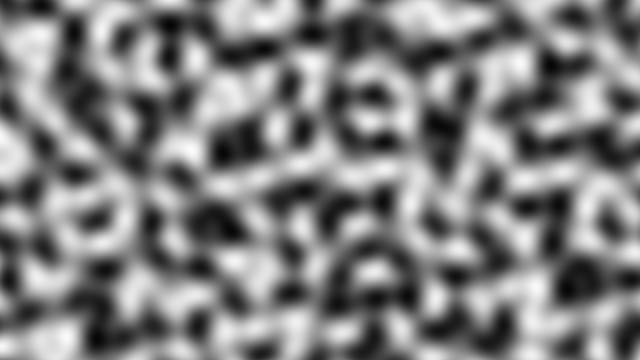
\includegraphics[width=\linewidth,trim=0bp 75bp 0bp 75bp,clip]{folien/bilder/demo-ziele/08-value-noise.png}\par
%{\scriptsize START = ZIEL aus Demo 5.}
\end{column}
\begin{column}{.30\textwidth}
{\small\bfseries 2 · Feine Details ergänzen}\par
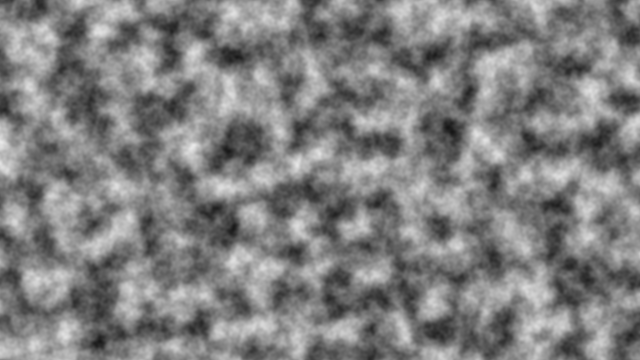
\includegraphics[width=\linewidth,trim=0bp 75bp 0bp 75bp,clip]{folien/bilder/demo-ziele/09-fbm-fbm.png}\par
{\scriptsize Mehrere Maßstäbe gewichtet überlagern.}
\end{column}
\begin{column}{.30\textwidth}
{\small\bfseries 3 · Wolkendichte und Farbe}\par
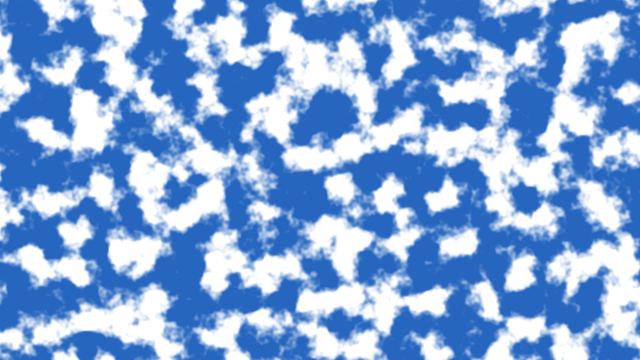
\includegraphics[width=\linewidth,trim=0bp 75bp 0bp 75bp,clip]{folien/bilder/demo-ziele/09-fbm.png}\par
{\scriptsize Blau und Weiß anhand der Dichte mischen.}
\end{column}
\end{columns}
{\small
\[F(p)=\frac{0{,}5N(p)+0{,}25N(2p)+0{,}125N(4p)+0{,}0625N(8p)}{0{,}9375}\]
\textbf{fBm:} Vier Oktaven: Frequenz verdoppeln, Gewicht halbieren. Die Division hält die Werte in $[0,1]$.\par
\textbf{Wolken:} $d=\operatorname{smoothstep}(0{,}4;\,0{,}65;\,F(p))$;
Farbe $=\operatorname{mix}(\text{Blau},\text{Weiß},d)$.\par
%\textbf{Bewegung erst im ZIEL:} $p\leftarrow p-(0{,}18;\,0{,}06)\,t$.
%Das vorhandene Muster wandert; es wird nicht pro Bild neu gewürfelt.}
}
%\editorauftrag{6}{09-fbm}{Ändert im ZIEL die Verschiebungsrichtung. In welche Richtung bewegen sich die Wolken?}
%\tafelverweis{8}{Maßstäbe, Wolkendichte und Animation}
\end{frame}
\endgroup
